\documentclass{article}
\usepackage[hidelinks]{hyperref}
\usepackage{graphicx}
\setlength{\parindent}{0pt}

\title{CKAS 6DOF User Manual}
\author{Tobias Brodel - Audiokinetic Experiments, RMIT University}

\begin{document}
	\maketitle
	\newpage

	\tableofcontents
	\newpage

	\section{Introduction}
	This manual details the operation of the 
	\href{http://www.ckas.com.au/6dof_low_cost_systems_62.html}{CKAS 
	Mechatronics W3s 6DOF motion platform} as it is used within the 
	Audiokinetic Experiments (AkE) labs at RMIT University. The structure of is 	a gradient from least technical to most technical -- most people will only 
	need to read \hyperref[playback]{Section 2} to get the system to play back 
	audiokinetic compositions. \hyperref[comp]{Section 3} deals with the 
	process for composing new works for the 6DOF and \hyperref[dev]{Section 4} 
	is useful for those who wish to contribute to software development in AkE.

	\section{Playback Operation}
	\label{playback}
	Playing back compositions is intended to be very simple. Tracks are loaded 
	into the system using a smartphone interface, then triggered when ready. 

	\subsection{Setup}
	Make sure the smartphone is on the same wireless network as the 6dof 
	system. Launch the TouchOSC application on the smartphone, choose the 
	``endroid" layout and make sure the host IP address is correct. If you need 
	help with network information ask whoever setup the rest of the 6DOF system.

	\subsection{TouchOSC Interface}
	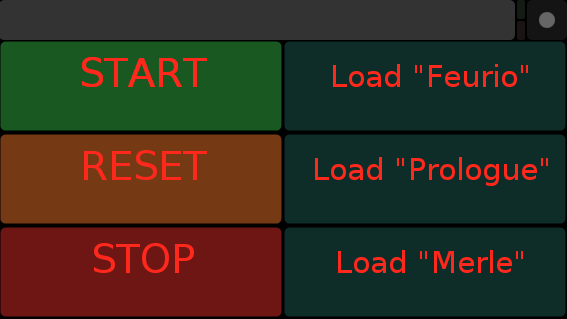
\includegraphics[width=\linewidth]{img/touchOSC.png}

	This is the interface you will use to load and play audiokinetic 
	compositions. A red light in the top right-hand corner will flash every 
	second or so to indicate that the 6DOF system is ready to load a track. If 
	this is not the case try hitting ``STOP", this should trigger the light.
	After you choose a track this light will momentarily stop flashing. It is 
	important to wait until it resumes before you continue, it should take a 
	couple of seconds. When ready hit the ``START" button. Once the track 
	finishes or you hit ``STOP" make sure to press ``RESET" to reposition the 
	motion simulator and ready the audio for the next track.

	\subsubsection{Quick Guide}
	\begin{enumerate}
		\item Make sure the red light is flashing by hitting ``STOP"
		\item Load a track
		\item When safe, hit the start button
		\item When the piece finishes hit ``RESET"
		\item If in doubt, hit ``STOP"
	\end{enumerate}

	\subsection{Troubleshooting}
	If the system becomes unresponsive check all network connections and try to 
	determine the correct IP addresses, update the TouchOSC coniguration if 
	necessary. If this doesn't work try to reboot the silver ``NUC" 
	microcomputer by holding down the power button. This should take 
	a couple of minutes. Next try powercycling the wireless router. If you 
	still have issues please contact AkE for technical assistance.

	\subsection{Maintenance}
	The TouchOSC interface relies on a ZTE smartphone with a specific layout 
	installed. Without this the installation will not run. Please ensure the 
	phone is charged every night.

	\section{Composition Interface}
	\label{comp}
	This section presumes you have a soundcard with 6 audio outputs and MIDI 
	out. The system has been tested in Pro Tools 10 and 11 but should work with
	any DAW.

	\subsection{Setup}
	The connection chain looks like this: \newline
	DAW -\textgreater soundcard -\textgreater midiout -\textgreater cubietruck 
	-\textgreater simcor \smallskip

	\subsubsection{MIDI}
	You will need to send CC data on channel 1 from your DAW. The following CC
	programs correspond to the 6 degrees of freedom.

	\begin{enumerate}
		\item  Modulation: X/Surge
		\item  Breath Controller: Y/Sway
		\item  Undefined: Z/Heave
		\item  Foot Controller: Pitch
		\item  Portamento Time: Roll
		\item  Data Entry (MSB): Yaw
	\end{enumerate}

	MIDI, having only 128 possible values, may not provide enough precision for 
	your composition. We have hacked around this by dedicating CC program 8 
	(Balance) as a smoothing parameter. This channel enables ``ramping" between 
	values, with a ramp time of between 50ms and 3 seconds. The setting is 
	global, not per channel. If set to zero the smoothing has no effect. Please 
	ensure that at the end of your composition, and at the end of your 
	sessions, that this value is reset to zero for the next user.

	Make sure your MIDI output is connected to the input of the USB MIDI 
	interface on the red ``Cubietruck" development board. If the network is set 
	up correctly CC data on channel one as described above should activate the 
	motion simulator.

	\subsubsection{Audio}
	This system is also designed to interact with synchronator projections and 	
	a transducer. The routing convention in AkE is as follows:

	\begin{enumerate}
		\item Headphones Left
		\item Headphones Right
		\item Transducer
		\item Synchronator Red
		\item Synchronator Green
		\item Synchronator Blue
	\end{enumerate}

	\subsection{Bouncing}
	Once your composition is finalised it needs to be bounced out for playback. 
	This means 6 mono 44.1kHz 16-bit .wav files and one .midi file. The naming 
	convention is as follows: 
	
	\begin{itemize}
		\item All lowercase
		\item Two tracks for headphones 
		\begin{itemize}
			\item left.wav
			\item right.rav
		\end{itemize}
		\item One track for transducer 
		\begin{itemize}
			\item trans.wav
		\end{itemize}
		\item Three tracks for synchronator
		\begin{itemize}
			\item red.wav
			\item green.wav
			\item blue.wav
		\end{itemize}
	\end{itemize}

	Each track should be exactly the same length as playback speed is 
	determined by the number of samples in a track. If you're not using some of 
	these tracks just copy some other bounce into its place. For example, if 
	you are using the headphones but not the transducer copy left.wav as 
	trans.wav. Each track should begin with a second or so of silence to 
	accomodate for resetting the motion simulator before playback. 

	\section{Software Development}
	\label{dev}
	The system is based on a custom \href{http://puredata.info}{Pure Data} 
	external implementing the ``Generic UDP Interface" for motion systems 
	designed by CKAS Mechatronics. For documentation contact AkE. The pd
	external, patches and source code can be found on github:

	\url{https://github.com/AkE-RMIT/ckas}\medskip

	The external is written in C following the KNF style guide: 
	
	\url{http://www.openbsd.org/cgi-bin/man.cgi/OpenBSD-current/man9/style.9?query=style}\medskip

	The pd patches are developed using the default packages from the Debian 
	repositories. \emph{Not} pd-extended. A path must be included to any 
	external you use as it may not be installed on the development boards in 
	the AkE labs.\medskip

	This manual itself is written in \LaTeX. As with everything else, patches 
	are welcome.\medskip

	All software is to be published under a BSD 2-Clause License:

	\url{http://opensource.org/licenses/BSD-2-Clause}

\end{document}
